\section{Research Method}
\label{ResearchMethod}
Explaining research chronological, including research design, research procedure (in the form of algorithms, Pseudocode or other), how to test and data acquisition. The description of the course of research should be supported references, so the explanation can be accepted scientifically.
\par
Tables and Figures are presented center, as shown below and cited in the manuscript.\\

\begin{table}[ht]
\caption{The Performance of ...}
\centering
\begin{tabular}{lcr}
\hline
Variable & Speed (rpm) & Power (kW) \\
\hline
x & 10 & 8.6 \\
y & 15 & 12.4 \\
z & 20 & 15.3 \\
\hline
\end{tabular}
\end{table}

\begin{figure}[ht]
\centering
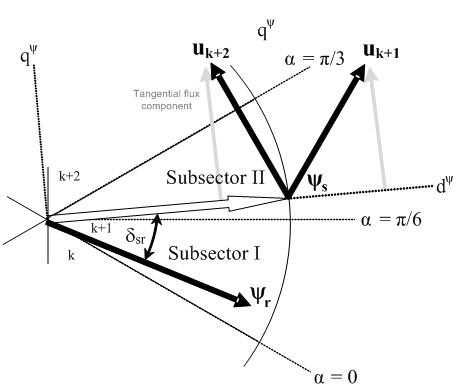
\includegraphics[scale=0.5]{figures/figure1}
\caption{Effects of selecting different switching under dynamic condition}
\end{figure}